% Diagrama 3: Flujo de la simulación en manet-jerarquica.cc
% Compilar con: lualatex flujo-simulacion.tex  (sale flujo-simulacion.pdf)
\documentclass[tikz,border=16pt]{standalone}
\usetikzlibrary{positioning,arrows.meta}
\usepackage{amsmath}
\begin{document}
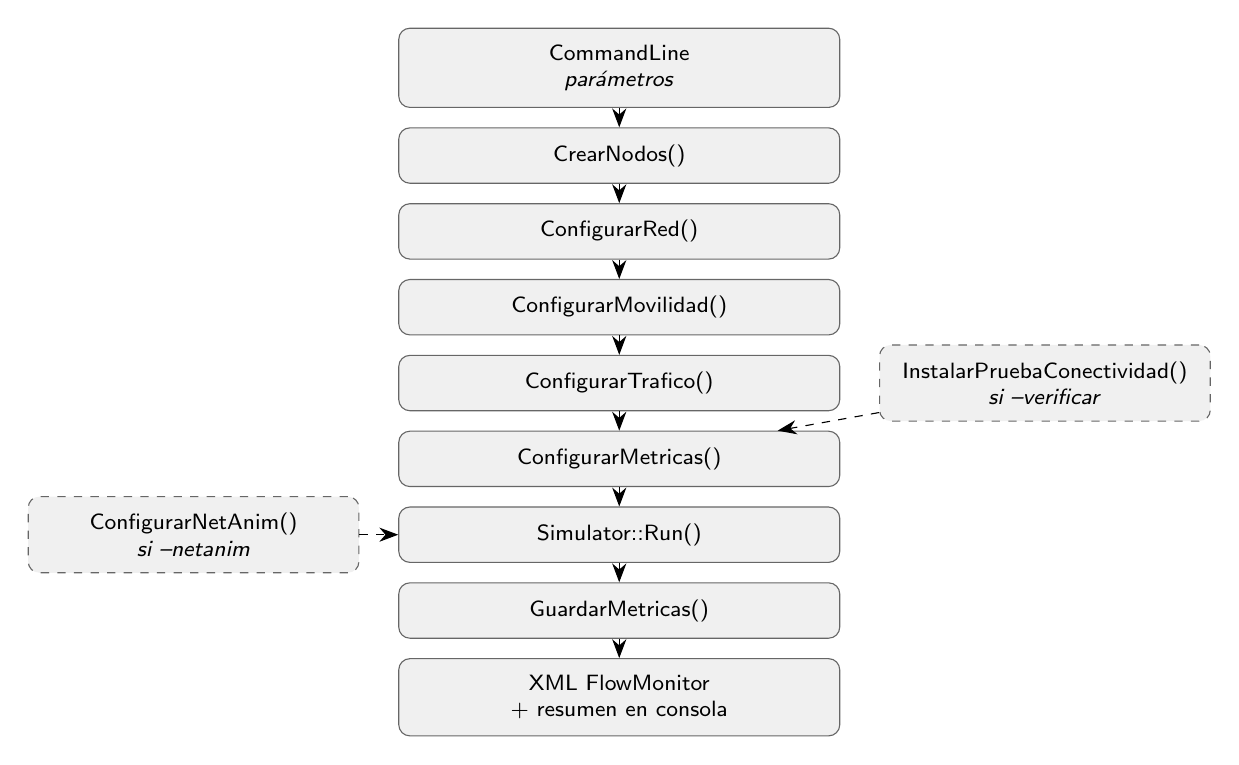
\begin{tikzpicture}[
  font=\sffamily\footnotesize,
  box/.style={draw=black!60, rounded corners=4pt, align=center,
              minimum width=5.6cm, inner sep=6pt, fill=black!6},
  side/.style={draw=black!60, dashed, rounded corners=4pt, align=center,
               minimum width=4.2cm, inner sep=6pt, fill=black!6},
  arr/.style={-{Stealth[length=2.4mm]}},
]
\node[box] (p)    {CommandLine\\ \textit{parámetros}};
\node[box] (cn)   [below=7pt of p]    {CrearNodos()};
\node[box] (cr)   [below=7pt of cn]   {ConfigurarRed()};
\node[box] (cm)   [below=7pt of cr]   {ConfigurarMovilidad()};
\node[box] (ct)   [below=7pt of cm]   {ConfigurarTrafico()};
\node[box] (cmt)  [below=7pt of ct]   {ConfigurarMetricas()};
\node[box] (run)  [below=7pt of cmt]  {Simulator::Run()};
\node[box] (guard)[below=7pt of run]  {GuardarMetricas()};
\node[box] (out)  [below=7pt of guard]{XML FlowMonitor\\ + resumen en consola};

\draw[arr] (p) -- (cn);
\draw[arr] (cn) -- (cr);
\draw[arr] (cr) -- (cm);
\draw[arr] (cm) -- (ct);
\draw[arr] (ct) -- (cmt);
\draw[arr] (cmt) -- (run);
\draw[arr] (run) -- (guard);
\draw[arr] (guard) -- (out);

% Rama --netanim (a la izquierda de Run)
\node[side] (anim) [left=14pt of run]
  {ConfigurarNetAnim()\\ \textit{si --netanim}};
\draw[arr, dashed] (anim) -- (run);

% Rama --verificar (a la derecha de tráfico/métricas)
\node[side] (ver) [right=14pt of ct]
  {InstalarPruebaConectividad()\\ \textit{si --verificar}};
\draw[arr, dashed] (ver) -- (cmt);
\end{tikzpicture}
\end{document}
